% !TEX root = main.tex
\documentclass[10pt,twocolumn]{article}
\newif\ifpaperdraft
\paperdrafttrue
\IfFileExists{metadata.tex}{% Human-supplied publication metadata belongs in this file only.
% Do not replace these author-supplied values with inferred identities.
\newcommand{\PaperTitle}{%
  From Position Samples to Executable Commands: Timing and Feasibility for
  Jerk-Limited Reference Following%
}
\newcommand{\PaperAuthorName}{\textit{Li Tang}}
\newcommand{\PaperAffiliation}{\textit{Independent Researcher}}
\newcommand{\PaperEmail}{\textit{timli0617@gmail.com}}
\newcommand{\PaperAuthorBlock}{%
  \PaperAuthorName\\
  \PaperAffiliation\\
  \PaperEmail%
}
\newcommand{\PaperPDFAuthor}{Li Tang}
\newcommand{\PaperDate}{}
}{\paperdrafttrue
\newcommand{\paperauthor}{Author metadata withheld from provisional draft}
\newcommand{\paperaffiliation}{Independent draft metadata entry}
\newcommand{\paperdate}{Provisional evidence snapshot}
\newcommand{\paperrepository}{Repository URL required for release build}
}
\usepackage[letterpaper,margin=0.75in,columnsep=0.25in]{geometry}
\usepackage[T1]{fontenc}
\usepackage{amsmath,amssymb,amsthm,mathtools}
\usepackage{newtxtext,newtxmath}
\usepackage{microtype}
\usepackage{graphicx}
\usepackage{booktabs}
\usepackage{tabularx}
\usepackage{siunitx}
\usepackage{xcolor}
\usepackage{enumitem}
\usepackage[numbers,sort&compress]{natbib}
\usepackage[hidelinks]{hyperref}
\usepackage[nameinlink,capitalise,noabbrev]{cleveref}

\definecolor{paperblue}{HTML}{17365D}
\definecolor{paperred}{HTML}{A61B1B}
\definecolor{papergray}{HTML}{5A6573}
\hypersetup{
  pdftitle={Terminal-State Mismatch Causes Stop-and-Go in Jerk-Limited Online Trajectory Generation},
  pdfsubject={Jerk-limited online trajectory generation and target-state contracts},
  colorlinks=true,
  linkcolor=paperblue,
  citecolor=paperblue,
  urlcolor=paperblue
}
\sisetup{detect-all,group-separator={,},group-minimum-digits=4}
\setlength{\emergencystretch}{2em}
\setlength{\parindent}{1em}
\setlength{\parskip}{0pt}
\raggedbottom

\newtheorem{theorem}{Theorem}
\newtheorem{corollary}{Corollary}
\newtheorem{proposition}{Proposition}
\newtheorem{lemma}{Lemma}
\theoremstyle{definition}
\newtheorem{definition}{Definition}
\theoremstyle{remark}
\newtheorem{remark}{Remark}

\crefname{theorem}{Theorem}{Theorems}
\crefname{corollary}{Corollary}{Corollaries}
\crefname{proposition}{Proposition}{Propositions}
\crefname{lemma}{Lemma}{Lemmas}
\crefname{figure}{Fig.}{Figs.}
\crefname{table}{Table}{Tables}

\newcommand{\claimtag}[1]{\ifpaperdraft\textsuperscript{\textcolor{papergray}{[#1]}}\fi}
\newcommand{\Ponly}{\textsc{P-only}}
\newcommand{\PV}{\textsc{PV}}
\newcommand{\PVA}{\textsc{PVA}}
\newcommand{\FutureOOne}{\textsc{Future-O1}}
\newcommand{\vcrit}{v_{\mathrm{crit}}}
\newcommand{\dcrit}{d_{\mathrm{crit}}}
\newcommand{\vref}{v_{\mathrm{ref}}}
\newcommand{\targetstate}{x^{\star}}
\newcommand{\R}{\mathbb{R}}
\newcommand{\abs}[1]{\lvert #1\rvert}
\newcommand{\norm}[1]{\lVert #1\rVert}
\newcommand{\paperdraftnotice}{%
  \ifpaperdraft
  \par\vspace{0.3em}\noindent
  \fcolorbox{paperred}{white}{\parbox{0.96\linewidth}{\centering\small\color{paperred}
  PROVISIONAL EVIDENCE DRAFT. Hash-pinned results are taken from manifests that report dirty git worktrees. This PDF is complete for review but is intentionally blocked from arXiv release.}}
  \par\vspace{0.5em}
  \fi
}

% Stable prose, method, dataset, and evidence-scope macros.
% Empirical result macros are generated separately in generated/numbers.tex.

% Product, API, and method identities.
\newcommand{\Ruckig}{\textsf{Ruckig}}
\newcommand{\OrdinaryRuckig}{ordinary \Ruckig}
\newcommand{\RuckigTrackingInterface}{\Ruckig{} Tracking Interface}
\newcommand{\TrackigAPI}{\texttt{Trackig}}
\newcommand{\TrackingAwareFollower}{tracking-aware follower}
\newcommand{\ExecutableTargetGovernor}{executable-target governor}
\newcommand{\DirectConstantJerkExecution}{direct constant-jerk execution}
\newcommand{\ViabilityShieldedRuckig}{viability-shielded \Ruckig}
\newcommand{\StateToStateOTG}{state-to-state online trajectory generator}
\newcommand{\PositionOnlyReferenceStream}{position-only reference stream}

% Experiment and dataset names.
\newcommand{\PhaseAAnalyticReferences}{Phase~A analytic references}
\newcommand{\DevelopmentCSV}{development CSV}
\newcommand{\FrozenVThreeProtocol}{frozen synthetic v3 protocol}
\newcommand{\PostfreezeCompatibilityRegression}{post-freeze compatibility regression}

% Evidence-scope labels. These describe provenance, not performance.
\newcommand{\CurrentEvidenceScope}{current evidence}
\newcommand{\FrozenEvidenceScope}{frozen-scope evidence}
\newcommand{\PostfreezeEvidenceScope}{post-freeze evidence}
\newcommand{\NegativeEvidenceScope}{current negative evidence}
\newcommand{\ExploratoryConfoundedScope}{exploratory, confounded evidence}
\newcommand{\NotEvaluatedScope}{not evaluated}

% Draft notes are opt-in and are disabled in normal builds.
\newif\ifdraftnotes
\draftnotesfalse
\newcommand{\DraftOnlyNote}[1]{%
  \ifdraftnotes
    \par\smallskip
    \noindent\colorbox{yellow!20}{%
      \parbox{\dimexpr\linewidth-2\fboxsep\relax}{%
        \textcolor{red!60!black}{\textbf{Draft note:} #1}%
      }%
    }
    \par\smallskip
  \fi
}

% Generated by paper/scripts/build_artifacts.py; do not edit.
\newcommand{\EvidenceProfile}{provisional}
\newcommand{\EFifteenGridCount}{2,144}
\newcommand{\EFifteenSobolCount}{128}
\newcommand{\EFifteenSeamCount}{16}
\newcommand{\EFifteenMaxBoundaryErrorPercent}{\num{0.0195}\%}
\newcommand{\ESixteenArmCount}{1,260}
\newcommand{\ESixteenWrongRipple}{\num{3.2007}}
\newcommand{\ESeventeenWorkConditionCount}{11}
\newcommand{\ESeventeenStressConditionCount}{6}
\newcommand{\ESeventeenStressPairCount}{720}
\newcommand{\ESeventeenPairPerCondition}{120}
\newcommand{\ESeventeenDevelopmentRowCount}{2,380}
\newcommand{\ESeventeenHoldoutRowCount}{14,280}
\newcommand{\ESeventeenWorkPairCount}{1,320}
\newcommand{\ESeventeenWeakMedianPercent}{\num{79.03}\%}
\newcommand{\ESeventeenWeakMinimumPercent}{\num{56.74}\%}
\newcommand{\ESeventeenStressMedianPercent}{\num{45.13}\%}
\newcommand{\ESeventeenStressMinimumPercent}{\num{-10.63}\%}
\newcommand{\ESeventeenStressImprovedCount}{119}
\newcommand{\ESeventeenSyntheticCount}{20}
\newcommand{\ESeventeenSyntheticWorstPercent}{\num{98.67}\%}
\newcommand{\RecordedSampleCount}{7,673}
\newcommand{\RecordedCycleCount}{7,672}
\newcommand{\RecordedDuration}{\num{76.72}\,s}
\newcommand{\RecordedBaselineRMSE}{\num{0.002951}\,rad}
\newcommand{\RecordedPVRMSE}{\num{0.002352}\,rad}
\newcommand{\RecordedPVReductionPercent}{\num{20.30}\%}
\newcommand{\RecordedPVALRMSE}{\num{0.003536}\,rad}
\newcommand{\RecordedPVAIncreasePercent}{\num{19.83}\%}
\newcommand{\RecordedPSubsampleLag}{\num{21.029}\,ms}
\newcommand{\RecordedPVLag}{\num{10}\,ms}
\newcommand{\RecordedPVSubsampleLag}{\num{9.554}\,ms}
\newcommand{\RecordedPVALag}{\num{10}\,ms}
\newcommand{\RecordedPVASubsampleLag}{\num{13.976}\,ms}
\newcommand{\RecordedDeadlineMissCount}{1}
\newcommand{\RecordedBestRMSE}{\num{0.002129}\,rad}
\newcommand{\RecordedBestReductionPercent}{\num{27.87}\%}
\newcommand{\RecordedBestSubsampleLag}{\num{9.740}\,ms}
\newcommand{\RecordedBestVsVendorReductionPercent}{\num{9.49}\%}
\newcommand{\RecordedBestLagTradeoff}{\num{0.186}\,ms}
\newcommand{\RecordedLocalPolyRMSE}{\num{0.003308}\,rad}
\newcommand{\RecordedDeadband}{\num{1e-10}\,rad\,s$^{-1}$}
\newcommand{\RecordedMinimumNonzeroTarget}{\num{2.705e-09}\,rad\,s$^{-1}$}
\newcommand{\RecordedZeroTargetCount}{2}
\newcommand{\PVAPVEquivalentCoordinateCount}{80}
\newcommand{\VmaxInteraction}{\num{0.0}}
\newcommand{\RuckigVersion}{0.17.3}


\title{Terminal-State Mismatch Causes Stop-and-Go in Jerk-Limited Online Trajectory Generation:\\A Dimensionless Boundary and a Causal Velocity-Target Remedy}
\author{\paperauthor\\\small\paperaffiliation}
\date{\paperdate}

\begin{document}
\maketitle
\paperdraftnotice

\begin{abstract}
Streaming a moving position reference into a jerk-limited online trajectory generator can produce severe within-period stop-and-go motion even when every sampled position is reached accurately. We show that the cause is a terminal-state mismatch: a position-only target implicitly requests zero terminal velocity and acceleration at every control tick, converting continuous motion into repeated rest-to-rest transfers. For a single third-order integrator with symmetric acceleration and jerk bounds, we derive the maximum one-period rest-to-rest displacement and express the transition through two dimensionless variables, $q=4A/(JT)$ and $\rho=\abs{\vref}/\vcrit$. The reachability boundary is $\rho=1$. We then prove that a matched velocity target admits a zero-jerk invariant continuation and give a causal fixed-grid construction from scheduled positions. In Ruckig~\RuckigVersion, E15 completes \EFifteenGridCount{} required cells and \EFifteenSobolCount{} numerical holdouts, while E16 isolates the derivative target in \ESixteenArmCount{} intervention arms. A frozen holdout shows improvement in all \ESeventeenWorkPairCount{} paired cells \testedEnvelope, while stronger stress diagnostics expose an explicit noise boundary. One recorded fixed-grid case reduces position RMSE by \RecordedPVReductionPercent{} and observed lag from 20 to 10 ms. The result is a scoped account of target-state semantics, not a universal claim about all online generators or tasks.
\end{abstract}

\section{Introduction}
\label{sec:introduction}

A sampled position stream can look accurate at its endpoints while being dynamically wrong between them. Consider a constant-speed reference sampled every control period. A follower sends the next position to a jerk-limited online trajectory generator (OTG), executes the first period of the resulting trajectory, and repeats. If every target silently includes zero terminal velocity and acceleration, the generator is not being asked to continue the motion. It is being asked to stop at every sample. When that stop is reachable within one period, the exact within-period solution is a short rest-to-rest pulse: accelerate, decelerate, arrive at the correct position, and reach zero velocity before the next command. Repetition produces \stopandgo{} motion even though the endpoint position error can be nearly zero. This is not feedback chattering, stick--slip, or a failure of jerk limitation. It is a mismatch between the intended continuous motion and the terminal derivatives carried by the command.\claimtag{C1}

This distinction matters in streaming robot interfaces. OTG algorithms are normally formulated for complete initial and target states under kinematic bounds. Ruckig, for example, accepts target position, velocity, and acceleration and computes jerk-limited trajectories to arbitrary target states~\cite{berscheid2021ruckig}. An application that supplies positions while leaving the derivative fields at zero has therefore made a substantive modeling choice, whether or not the API makes that choice visually prominent. The resulting artifact may be missed by a benchmark based only on target-time position root-mean-square error (RMSE). It is visible in the exact piecewise-jerk profile, in the within-period velocity minimum and ripple, and in the repeated terminal stops.

The phenomenon raises three questions that are not answered by the instruction to ``set target velocity.'' First, when is a one-period rest-to-rest move reachable under acceleration and jerk limits? Without that boundary, the occurrence of the artifact appears parameter-specific. Second, does a matched velocity target remove the mechanism because it carries the correct state semantics, or merely because it provides another tunable input? Third, can the velocity be constructed causally from a scheduled position stream, and over what noise and timing envelope does that construction remain useful? These questions lead to a theory--experiment separation that is central to this paper. The theory concerns a single third-order integrator and proves reachability or feasible continuation. The experiments characterize how one pinned implementation, Ruckig~\RuckigVersion, realizes those possibilities. No theorem asserts that every OTG uses the same profile-selection policy.

We derive the maximum displacement of a symmetric jerk- and acceleration-limited rest-to-rest transfer in one control period. With period $T$, bounds $A$ and $J$, and reference speed $\vref$, the result reduces to two dimensionless variables,
\begin{equation}
 q=\frac{4A}{JT}, \qquad
 \rho=\frac{\abs{\vref}}{\vcrit}.
 \label{eq:intro-dimensionless}
\end{equation}
The boundary $\rho=1$ separates one-period rest-to-rest reachability from nonreachability when the velocity bound is inactive. The formula also gives a counterintuitive design implication: increasing $A$, $J$, or $T$ weakly enlarges the set of speeds for which repeated stopping is reachable. Looser dynamic limits can therefore expose, rather than cure, a bad terminal-state contract.\claimtag{C2}

The structural remedy is equally simple to state and more precise than a tuning heuristic. If the current state is $(p_k,\vref,0)$ and the next target is $(p_k+\vref T,\vref,0)$, then constant velocity with zero acceleration and jerk is an exact feasible continuation. We call this a \matchedvelocity. Its importance is not that velocity is always the best extra field, but that the terminal state is consistent with the invariant motion the application intends. We further specify a fixed-grid information contract in which $P[k+1]$ is an already scheduled target, while measurements are available only through index $k$. Under that contract, \FutureOOne{} constructs a target velocity from $P[k],P[k-1],P[k-2]$ without reading a future measurement.\claimtag{C3}\claimtag{C5}

The empirical program is organized by hypotheses rather than by experiment chronology. A boundary study completes \EFifteenGridCount{} required cells and \EFifteenSobolCount{} out-of-grid threshold searches; it confirms the dimensionless transition away from an explicitly reported set of \EFifteenSeamCount{} exact-seam numerical failures. A causal intervention study executes \ESixteenArmCount{} arms, varying the velocity coefficient and comparing wrong-sign, random-sign, position-lookahead, and minimum-duration alternatives. Only the matched velocity interventions reproduce the preregistered exact profile in every tested primary cell. A frozen robustness study then evaluates a development-selected causal observer on \ESeventeenWorkPairCount{} paired seed--configuration cells across 11 declared conditions. The weakest declared condition still has a median ripple reduction of \ESeventeenWeakMedianPercent, while six stronger, out-of-envelope diagnostics expose a failure boundary rather than being hidden. Finally, one recorded fixed-grid trajectory provides an engineering case study: PV \FutureOOne{} reduces RMSE by \RecordedPVReductionPercent{} and the \observedlag{} from 20 to \RecordedPVLag. A timestamp-aware local-polynomial replay does not improve the irregular-timestamp version, and that negative result remains part of the main account.\claimtag{C4}\claimtag{C6}\claimtag{C9}\claimtag{C13}

The contributions are fourfold:
\begin{enumerate}[leftmargin=*,itemsep=2pt]
  \item a closed-form one-period rest-to-rest reachability boundary, its $q$--$\rho$ normalization, and monotonic design consequences under explicit assumptions;
  \item a proof that the matched PV contract admits an invariant zero-jerk continuation, separated from empirical claims about a particular solver;
  \item exact-profile causal ablations and frozen holdout tests that reject several competing explanations and state both a tested work envelope and its observed boundary; and
  \item a reproducible recorded case study that distinguishes waveform tracking, observed lag, numerical guardrails, and best-tested constraint selection.
\end{enumerate}

The scope is deliberately narrower than a deployment claim. The theory is single-axis. The experiments are software evaluations without plant dynamics or multi-axis synchronization. The recorded evidence contains one waveform, and measured offline-host execution time is not a real-time schedulability result. These limits let the central causal claim remain testable: a position endpoint can be correct while its derivative contract makes the continuous motion wrong.

The remainder of the paper reviews OTG, reference shaping, and causal derivative estimation; defines the receding information contract and metrics; develops the dimensionless analysis; presents the boundary, ablation, robustness, and recorded results; and closes with limitations and implications for streaming motion interfaces.


\section{Related work}
\label{sec:related-work}

\subsection{Jerk-limited online trajectory generation}

% CLAIM: C01,C02,C11
Jerk-limited trajectory generation has a long lineage in real-time robot
motion.  Polynomial and synchronized constructions bound higher derivatives
while moving between specified states
\citep{MacfarlaneCroft2003JerkBounded,HaschkeEtAl2008Online}.
Discrete-time filtering provides another route to trajectories with bounded
velocity, acceleration, and jerk
\citep{GerelliLoBianco2010DiscreteFilter}, while mathematical programming can
optimize a minimum-jerk criterion under constraints
\citep{CanaliEtAl2014MinimumJerk}.  Path-accurate schemes address preservation
of a known desired path under jerk limits
\citep{LangeAlbuSchaeffer2016PathAccurate}.  These objectives should not be
collapsed: terminal-state interpolation, path preservation, minimum-jerk
optimization, and following an incompletely observed moving reference are
different problems.

\Ruckig{} generates time-optimal jerk-limited trajectories to arbitrary target
states and exposes a real-time state-to-state update interface
\citep{BerscheidKroeger2021Ruckig}.  That capability is the native follower in
our ordinary state-to-state conditions.  The distinction developed here lies
upstream and at the execution boundary: a position stream does not itself
define a time-aligned target state, and the legality of the executed
control-period prefix depends on its full piecewise profile.  We make no
priority claim for either observation.

\subsection{Reference governance and predictive motion}

% CLAIM: C02,C09
Reference and command governors are add-on mechanisms that modify references
to enforce constraints for a specified plant or closed-loop model
\citep{KolmanovskyEtAl2014GovernorTutorial,GaroneEtAl2017GovernorSurvey}.
This perspective motivates the term \emph{executable-target governor}: the
layer is neither an estimator nor a replacement for the native trajectory
solver.  Our construction is substantially narrower than general governor
theory.  It uses uncoupled sampled triple-integrator command dynamics and a
one-period viability check; it does not inherit robust plant-level,
disturbance, or stability guarantees from the broader literature.

Receding-horizon optimization can combine target updates, jerk-input
kinematics, and constraints over a longer prediction window
\citep{GhazaeiArdakaniEtAl2015MPC}.  Such a formulation can trade tracking,
effort, and future feasibility jointly.  The present method instead selects a
single adjacent jerk from analytically constructed candidate intervals and
checks the resulting next state.  It is intended to make the timing and
command contract explicit, not to claim MPC-equivalent optimality.

\subsection{Position-only state estimation and timing}

% CLAIM: C05
Derivatives from sampled positions can be obtained by local-polynomial
smoothing and differentiation \citep{SavitzkyGolay1964}, fixed-gain
\(\alpha\)--\(\beta\)--\(\gamma\) trackers
\citep{Kalata1984TrackingIndex,SahoMasugi2015ABG}, or state-space filtering and
prediction \citep{Kalman1960Filtering}.  Recent work on real-time numerical
differentiation emphasizes the distinction between estimates that use data
available at the estimated time and noncausal methods that consume future
samples \citep{VermaEtAl2024Differentiation}.  Our experiments do not propose
a new estimator.  They use simple derivative sources as controlled
information conditions and retain both represented time and availability time
through the downstream pipeline.

This bookkeeping matters because filtering delay and prediction horizon
compose.  A posterior representing \(t_{k-1}\) but available at \(t_k\) must
first be propagated to the control time before a prediction \(h\) beyond
\(t_k\) has its stated meaning.  Relabeling a delayed posterior as current
state does not create information; a model-based propagation must be explicit.
Similarly, a centered stencil aligned at \(t_k\) is an offline condition if it
requires \(p_{k+1}\).

\subsection{Moving-reference interfaces and method identity}

% CLAIM: C02,C12
The official \RuckigTrackingInterface{} documentation describes an interface
that predicts ahead to reduce lag when following a sampled signal, and the API
reference identifies the corresponding \TrackigAPI{} class
\citep{RuckigTrackingTutorial,RuckigTrackigAPI}.  We cite these sources only to
establish that moving-signal following is recognized as a distinct interface
behavior.  The interface was not measured in this project; the evidence does
not show that it is necessary, superior, or available in every tested
binding.

\begin{table}[t]
  \centering
  \small
  \caption{Conceptual method taxonomy.  Target information and the actually
  executed follower are independent factors.  ``Exact prefix'' means exact
  segment data are exposed; otherwise internal jerk remains unavailable.}
  \label{tab:method-taxonomy}
  \setlength{\tabcolsep}{4pt}
  \begin{tabular}{p{0.20\linewidth}p{0.18\linewidth}p{0.20\linewidth}p{0.27\linewidth}}
    \toprule
    Method role & Reference information & Executed profile & Identity boundary \\
    \midrule
    Ordinary state-to-state OTG & terminal P/PV/PVA request & native
    piecewise prefix & unshielded native command \\
    Tracking-aware follower & sampled/predicted moving reference & interface
    dependent & not evaluated here \\
    Viability-shielded OTG & governed or native candidate & native or
    replacement & shield decision changes identity \\
    Direct governor execution & future objective plus current state & one
    exact constant-jerk segment & governor action is the command \\
    \bottomrule
  \end{tabular}
\end{table}

The synthesis in \cref{tab:method-taxonomy} is the gap this paper addresses:
the same P/PV/PVA label may feed different governors or followers, and the same
declared follower may be replaced on execution.  Consequently, a defensible
comparison needs both an information condition and an executed-method
identity.  The following formulation makes those two axes, and every relevant
clock, explicit.

\section{Problem Formulation and Information Contract}
\label{sec:problem}

\subsection{Kinematic model and fixed-period follower}

We consider one translational or rotational coordinate with state $x=(p,v,a)$ and control $j$,
\begin{equation}
 \dot p=v,\qquad \dot v=a,\qquad \dot a=j,
 \label{eq:third-order}
\end{equation}
subject to symmetric bounds
\begin{equation}
 \abs{v(t)}\le V,\qquad \abs{a(t)}\le A,\qquad \abs{j(t)}\le J.
 \label{eq:bounds}
\end{equation}
The control period is $T$. At tick $k$, the follower initializes the OTG from the state produced at the end of the preceding tick, supplies a target state, commits one period of the returned trajectory, and repeats. The generator may compute a trajectory whose free duration exceeds $T$; our mechanism analysis nevertheless inspects exactly what is executed on $[kT,(k+1)T]$.

Let $P[k]$ denote the scheduled position at time $kT$. A constant-speed schedule satisfies
\begin{equation}
 P[k+1]-P[k]=\vref T.
 \label{eq:constant-schedule}
\end{equation}
The operational distinction is not whether the position is current or one step ahead; it is which complete state accompanies that position. We study three target contracts:
\begin{align}
 \Ponly &: \targetstate_{k+1}=(P[k+1],0,0), \label{eq:p-contract}\\
 \PV &: \targetstate_{k+1}=(P[k+1],\widehat V[k+1],0), \label{eq:pv-contract}\\
 \PVA &: \targetstate_{k+1}=(P[k+1],\widehat V[k+1],\widehat A[k+1]). \label{eq:pva-contract}
\end{align}
For constant motion, the matched values are $\widehat V[k+1]=\vref$ and $\widehat A[k+1]=0$. Thus matched PVA carries no additional physical information beyond matched PV in that special case; it is retained as a negative control, not dismissed for general motion.\claimtag{C8}

\begin{figure*}[t]
 \centering
 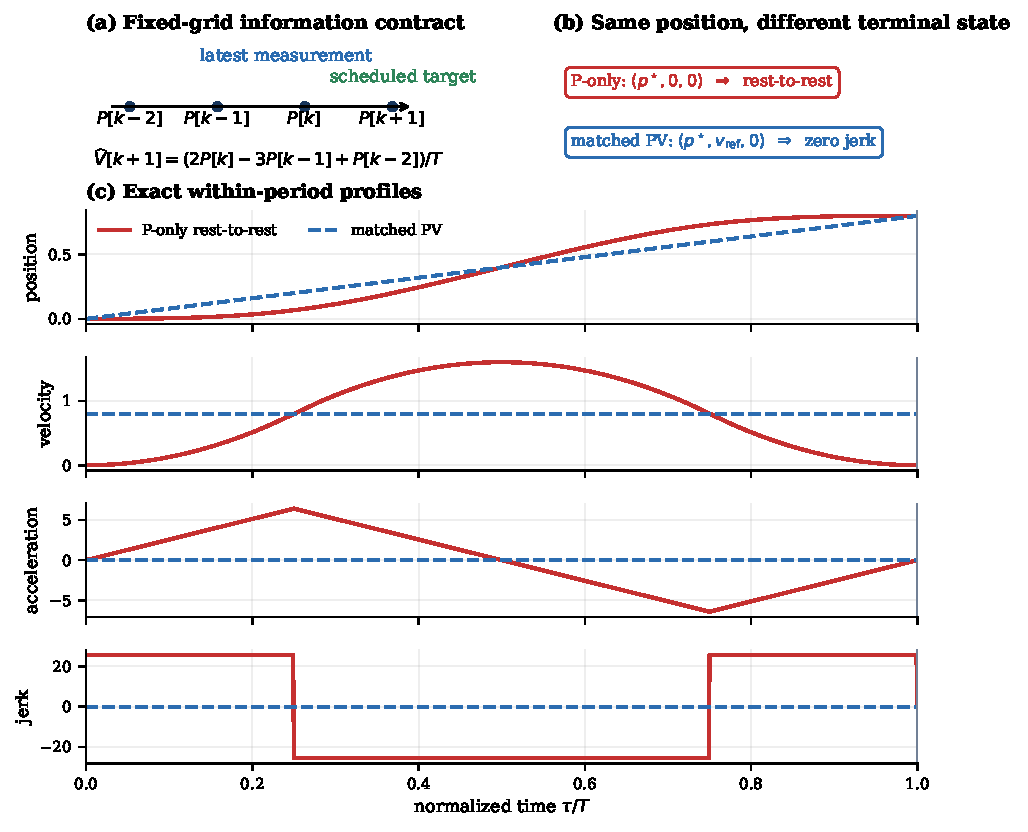
\includegraphics[width=\textwidth]{figures/generated/fig1_mechanism_profiles.pdf}
 \caption{Mechanism and information contract. (a) At tick $k$, $P[k+1]$ is an already scheduled target; measurements are available only through $P[k]$. (b) Identical position targets encode different terminal states. (c) A representative feasible P-only transfer reaches the correct endpoint after a rest-to-rest pulse, whereas matched PV admits constant velocity and zero jerk. The profiles are analytic normalized examples, not measured robot signals.}
 \label{fig:mechanism}
\end{figure*}

\subsection{Scheduled target versus future measurement}

The indexing in \cref{eq:pv-contract} can otherwise invite a noncausal interpretation. We define the information available when constructing the target for interval $[kT,(k+1)T]$ as
\begin{equation}
 \mathcal I_k=\{P[k+1]\text{ scheduled};\ P[k],P[k-1],P[k-2]\text{ available}\}.
 \label{eq:information-set}
\end{equation}
The semicolon is important. The target scheduler has already made $P[k+1]$ available, but no measurement after time $kT$ is observed. A predictor that reads only the history through $P[k]$ is causal under this contract even though its output is associated with the scheduled target at $k+1$. This is the timeline shown in \cref{fig:mechanism}a.

Our fixed-grid \FutureOOne{} velocity target is
\begin{equation}
 \widehat V[k+1]=\frac{2P[k]-3P[k-1]+P[k-2]}{T}.
 \label{eq:future-o1}
\end{equation}
The name describes the one-step target association used by the implementation; it does not mean that $P[k+1]$ is used as a future measurement. Startup samples use the explicitly reported fallback in the experiment specification. E17's irregular-timestamp replay deliberately rejects \cref{eq:future-o1} when the prediction horizon is not exactly one nominal step, rather than silently applying a fixed-step formula to a different contract.\claimtag{C5}\claimtag{C13}

\subsection{Mechanism metrics}

Endpoint position error is insufficient to identify \stopandgo. For every committed interval, the experiment reconstructs the exact piecewise-constant-jerk profile returned by the solver and evaluates it within the period. The primary mechanism readouts are: rest-to-rest pulse fraction, endpoint-stop fraction, stop-and-go event rate, velocity ripple normalized by $\abs{\vref}$, the lower tail of within-period $\abs v/\abs{\vref}$, and the fraction of cycles containing near-zero velocity. A profile-exact flag records whether the candidate matches the preregistered invariant profile within numerical tolerance. Constraint violations, fallbacks, solver failures, and incomplete cycles are guardrails.

For a constant reference, normalized velocity ripple is the range of the exact within-period velocity divided by $\abs{\vref}$. It is zero for the constant-velocity continuation and positive for an acceleration--deceleration pulse. The near-zero and endpoint-stop metrics distinguish a profile that merely varies around $\vref$ from one that actually stops. E15 and E16 therefore do not infer the mechanism from RMSE or from a target field alone.

\subsection{Recorded waveform metrics}

The recorded case uses raw-time position RMSE after a fixed startup exclusion, integer cross-correlation lag on the 10 ms grid, and a local quadratic sub-sample refinement. We call both lag quantities \observedlag{} because they describe alignment between two waveforms. They do not measure computation time, communication delay, or closed-loop wall-clock latency. Target projection and kinematic limit checks are scientific guardrails. Per-cycle execution time and deadline misses are reported separately as offline-host diagnostics.

The recorded input contains \RecordedSampleCount{} samples over \RecordedDuration. It is one trajectory on one axis, not a population of tasks. Comparisons within A04 and A06 use the same velocity-limited waveform; we do not form causal performance ratios between the current-online baseline and a candidate produced from a different input waveform. These restrictions define the scope of the recorded case study before any result is examined.\claimtag{C9}\claimtag{C10}


\section{Dimensionless Analysis and Matched-Velocity Invariance}
\label{sec:analysis}

\subsection{One-period rest-to-rest reachability}

Translate the initial position to zero and consider positive displacement; the negative case follows by sign reversal. The terminal conditions are
\begin{equation}
 p(0)=0,quad v(0)=a(0)=0,qquad v(T)=a(T)=0.
 \label{eq:rest-boundary-conditions}
\end{equation}
We first exclude an active velocity bound and return to its sufficient condition in the theorem statement.

\begin{theorem}[One-period rest-to-rest displacement]
\label{thm:rest-boundary}
For the system in \cref{eq:third-order,eq:bounds} with the boundary conditions in \cref{eq:rest-boundary-conditions}, suppose the position is unconstrained and $V\ge2\vcrit$. The maximum reachable absolute displacement in duration $T$ is
\begin{equation}
 \dcrit=T\vcrit,
 \qquad
 \vcrit=
 \begin{cases}
 \displaystyle \frac{JT^2}{32}, & A\ge \dfrac{JT}{4},\\[6pt]
 \displaystyle \frac{AT}{4}-\frac{A^2}{2J}, & A<\dfrac{JT}{4}.
 \end{cases}
 \label{eq:vcrit}
\end{equation}
Every displacement $d$ satisfying $\abs d\le\dcrit$ is reachable with $v(T)=a(T)=0$.
\end{theorem}

\begin{proof}[Proof sketch]
The reachable set at fixed $T$ is convex and the terminal displacement is a linear functional of the jerk. Pontryagin's maximum principle, including acceleration-boundary arcs, therefore places an extremizer at $j\in\{-J,0,J\}$ with $a\in\{-A,A\}$ whenever the corresponding state bound is active~\cite{pontryagin1962maximum}. Time reversal and sign reflection give an extremal acceleration that is nonnegative on the first half, nonpositive on the second, and antisymmetric about $T/2$. On $[0,T/2]$ its pointwise upper envelope is obtained by ramping from zero with $+J$, respecting $A$, and ramping back to zero with $-J$ in time to mirror the deceleration half.

If $A\ge JT/4$, the acceleration is triangular, with four equal jerk segments $+J,-J,-J,+J$ of duration $T/4$. The midpoint velocity is $JT^2/16$. If $A<JT/4$, let $h=A/J$; the first half contains a ramp of duration $h$, an acceleration plateau of duration $T/2-2h$, and a ramp down of duration $h$, yielding midpoint velocity $AT/2-A^2/J$. The optimal velocity profile is symmetric, and its integral is $T/2$ times the midpoint velocity, which gives \cref{eq:vcrit}. Thus the maximum speed on the profile is $2\vcrit$, explaining the sufficient condition on $V$. Scaling the signed jerk and resulting state by $\abs d/\dcrit$ constructs every smaller displacement. A complete upper-bound and segment-integration argument appears in \cref{app:proofs}.
\end{proof}

The theorem is a reachability result. It identifies a feasible extremal rest-to-rest transfer and proves that a larger one is impossible under the stated assumptions. It does not specify which feasible profile an arbitrary OTG selects, nor does it cover an active velocity limit, asymmetric bounds, position constraints, plant dynamics, or multiple synchronized axes.

\subsection{Dimensionless boundary}

Substituting $q=4A/(JT)$ into \cref{eq:vcrit} gives
\begin{equation}
 \frac{\vcrit}{JT^2}=g(q)=
 \begin{cases}
 \dfrac{2q-q^2}{32}, & 0<q<1,\\[4pt]
 \dfrac{1}{32}, & q\ge1.
 \end{cases}
 \label{eq:gq}
\end{equation}
The two branches and the E15 phase coordinates are shown in \cref{fig:dimensionless-boundary}. The function and its first derivative are continuous at $q=1$, while the active profile topology changes from acceleration-limited to jerk-limited.

\begin{figure*}[t]
 \centering
 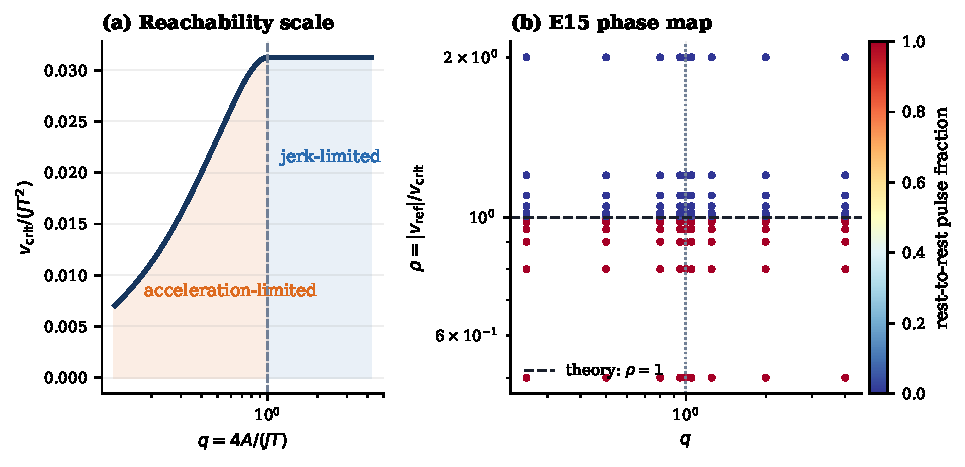
\includegraphics[width=\textwidth]{figures/generated/fig2_dimensionless_boundary.pdf}
 \caption{Dimensionless prediction. (a) The normalized critical speed has an acceleration-limited branch for $q<1$ and a saturated jerk-limited branch for $q\ge1$. (b) E15 configurations colored by observed rest-to-rest pulse fraction. The horizontal line $\rho=1$ is theoretical; the solver realization is empirical.}
 \label{fig:dimensionless-boundary}
\end{figure*}

\begin{corollary}[Dimensionless rest-to-rest boundary]
\label{cor:rho-boundary}
For the constant schedule in \cref{eq:constant-schedule}, a P-only transfer over one tick requires displacement $\abs{\vref}T$. Under the assumptions of \cref{thm:rest-boundary}, this transfer with terminal $v=a=0$ is reachable if and only if
\begin{equation}
 \rho=\frac{\abs{\vref}}{\vcrit}\le1.
 \label{eq:rho-boundary}
\end{equation}
\end{corollary}

If an OTG exactly completes that reachable P-only transfer and the next tick begins from its terminal rest state, repeated application produces a sequence of rest-to-rest pulses. That conditional statement explains the mechanism. The stronger statement that Ruckig~\RuckigVersion{} realizes this transition over the tested grid is established only by E15 in \cref{sec:boundary-results}. At the exact seam, numerical behavior is explicitly treated as diagnostic rather than absorbed into the theorem.\claimtag{C1}\claimtag{C2}

\begin{corollary}[Monotonic design implication]
\label{cor:monotonic}
For fixed values of the other quantities, $\vcrit$ is nondecreasing in $A$, $J$, and $T$. Hence increasing a limit or lengthening the control period weakly decreases $\rho$ for a fixed $\vref$ and can enlarge the one-period rest-to-rest region.
\end{corollary}

The dependence saturates in $A$ once $A\ge JT/4$, but it is otherwise strict. This is why limit tuning is not a reliable semantic repair: a seemingly more capable generator can become more capable of satisfying the unintended stop request.

\subsection{Matched-velocity continuation}

\begin{proposition}[Matched-PV invariant continuation]
\label{prop:matched-pv}
Suppose the current state lies on a constant-speed reference, $(p_k,\vref,0)$, with $\abs{\vref}\le V$. For target $(p_k+\vref T,\vref,0)$, the trajectory
\begin{equation}
 p(\tau)=p_k+\vref\tau,qquad
 v(\tau)=\vref,qquad a(\tau)=j(\tau)=0
 \label{eq:matched-continuation}
\end{equation}
for $0\le\tau\le T$ is feasible and exactly reaches the target.
\end{proposition}

\begin{proof}
Direct substitution satisfies the dynamics, endpoint state, and all acceleration and jerk bounds. The velocity bound follows from $\abs{\vref}\le V$.
\end{proof}

The proposition establishes existence, not solver preference or uniqueness under an unspecified objective. In E16, matched/oracle PV empirically reproduces this exact zero-ripple profile in every tested primary cell. In contrast, the P-only requirement $v(T)=0$ is structurally incompatible with \cref{eq:matched-continuation} whenever $\vref\ne0$.\claimtag{C3}

\begin{lemma}[Fixed-grid causality and affine exactness]
\label{lem:future-o1}
Under the information set in \cref{eq:information-set}, \FutureOOne{} in \cref{eq:future-o1} is causal. If $P[k]=c_0+c_1kT$, then $\widehat V[k+1]=c_1$ exactly.
\end{lemma}

\begin{proof}
The expression reads only samples with indices at most $k$. Substituting the affine sequence gives
$2(c_0+c_1kT)-3(c_0+c_1(k-1)T)+(c_0+c_1(k-2)T)=c_1T$.
\end{proof}

The lemma does not imply noise optimality, validity on an irregular grid, or superiority for arbitrary trajectories. Those are empirical questions, and the observer selected in the synthetic robustness experiment differs from the one selected for the recorded fixed-grid case.\claimtag{C5}


\section{Experimental protocol}
\label{sec:protocol}

The empirical study is organized as five evidence programs with different
information conditions and different inferential roles.  Phase~A isolates
target-state information on analytic references and records derivative-timing
diagnostics.  A single position trace supplies development-only negative
evidence for unfiltered finite-difference pipelines.  Frozen v3 artifacts
support a synthetic command-profile and runtime audit of the direct method.
A fresh, frozen V4 attempt supplies a same-follower P/PV/PVA comparison but
failed a preregistered validity gate and is non-confirmatory.  Finally,
post-freeze checks cover implementation compatibility and profile semantics,
but are not a new locked comparison.  Results from these programs are not
pooled.

\subsection{Phase~A: analytic information and timing controls}

% CLAIM: C03,C04
All Phase~A runs use one degree of freedom, a control period of
\SI{\ControlPeriodMS}{\milli\second}, and limits
\SI{\VelocityLimit}{\radian\per\second},
\SI{\AccelerationLimit}{\radian\per\second\squared}, and
\SI{\JerkLimit}{\radian\per\second\cubed}.  There is no look-ahead, the
minimum requested duration is one control period, and the interface convention
is \(\mathrm{target}[k]\mapsto\mathrm{output}[k+1]\).  The output of one
\OrdinaryRuckig{} update becomes the current state of the next update.  The
three smooth analytic references---a quadratic with an extremum, a cubic, and
a sinusoid---were pre-specified in the repository before the checked-in
aggregate result.  This provenance does not imply a formal pre-registration:
the generation manifest records a dirty worktree, and per-cycle outputs for most
non-P conditions were not retained.

The controlled target-component comparison uses P,
\([p_k,0,0]\), analytic PV truth, \([p_k,v_k^\star,0]\), and analytic PVA
truth, \([p_k,v_k^\star,a_k^\star]\).  The analytic derivatives are oracle
information, not estimates recoverable online from the position stream.  PV
and PVA truth request the same endpoint position and velocity at every tick;
they differ only in requested endpoint acceleration.  Consequently, their
comparison addresses the recorded position endpoint under this protocol.  It
does not test acceleration-estimator quality, internal-profile quality, or
control effort.

% CLAIM: C05,C08
A second Phase~A block distinguishes derivative formula accuracy from
availability.  Backward differences use history only.  A standard centered
estimate labelled at \(t_k\) uses \(p_{k+1}\) and is therefore an offline,
noncausal diagnostic.  A causal centered variant waits one sample, estimates
the state represented at \(t_{k-1}\), and then propagates that estimate to the
latest sample using the stated finite-difference model.  A separate
next-cycle analytic PVA oracle supplies the state belonging to \(t_{k+1}\) to
the update at \(k\).  It consumes one future sample and is used only as a
timing and indexing sanity control.

Position-following metrics are computed over the common interval beginning
after \PhaseACommonWarmupSamples{} warm-up samples and ending before sample
\PhaseAEvaluationStopIndex.  RMSE and maximum
absolute error compare output position with the reference at the recorded
output index.  The reported best lag is the integer-grid shift, searched over
the registered range, that minimizes aligned position RMSE; positive lag
means that output is late.  It is an end-to-end summary and must not be read
as estimator group delay.  Derivative RMSE uses a separate common interior
that removes estimator-specific endpoint rules.

\subsection{Development CSV}
\label{sec:protocol-csv}

% CLAIM: C06,C07,N01
The position CSV contains \CSVRowCount{} rows.  Only its \texttt{value} column is used:
elapsed time, timestamp, and topic fields are ignored, and every row is
assigned the same \SI{\ControlPeriodMS}{\milli\second} interval.  Evaluation
uses samples
\([\PhaseAEvaluationStartIndex,\CSVRowCount)\).  The trace has no registered velocity or
acceleration truth and is a development input, not an independent locked test
or a robot experiment.

The CSV matrix comprises P and unfiltered finite-difference-derived PV and PVA
pipelines using backward, offline-centered, and delayed causal-centered
derivatives.  Each row retains its causal/future-sample label.  Raw targets are
recorded before a fixed admissibility-projection function; projected targets
are then followed by \OrdinaryRuckig.  Projection is therefore part of the
tested pipeline when it triggers.  Because projection is not crossed as an
independent factor, this design cannot identify separate causal effects for
differentiation and projection.  Raw differentiated acceleration and
projection flags are target diagnostics, not measured plant acceleration or
executed-motion violations.

\subsection{Frozen synthetic v3 evidence}
\label{sec:protocol-v3}

% CLAIM: C10,C13
The v3 result layer is immutable and was not rerun for this paper draft.  It
retains whole-trajectory identities, explicit failure records, checksums, and
independently recomputed bounded summaries.  The locked-test denominator is
\VThreeTrajectoryCount{} complete synthetic trajectories.  The direct condition carrying the
frozen label \texttt{one\_step\_governed\_pva\_direct} contributes
\VThreeDirectCycleCount{} command cycles to the continuous V/A/internal-J,
point-admissibility, reachability, projection, and fallback audit.  Adjacent
sequence consistency has a smaller denominator because each trajectory
contributes one fewer transition than command states.

The registered continuous-constraint test accepts a margin no smaller than
\(\VThreeAuditTolerance\) in the corresponding physical unit.  Thus a recorded margin of
zero passes but is not strictly positive.  The audit concerns exact
constant-jerk command profiles in the synthetic triple-integrator protocol; it
does not include robot dynamics, torque, communication, collision, or
hardware execution.

Runtime uses a separately defined population.  After
\VThreeRuntimeWarmupSamples{} warm-up samples per
trajectory, \VThreeRuntimeCycleCount{} locked-test cycles remain for the same
frozen method label.  End-to-end runtime is compared with the
\SI{\ControlPeriodMS}{\milli\second} control period and summarized by empirical
quantiles, maximum, and deadline-miss count.  These are measurements from one
recorded Python environment, not worst-case execution-time bounds.  The
safety denominator and runtime denominator are never substituted for one
another.

The artifact program records \VThreeRawBundleCount{} independently verified
raw bundles and \VThreeBoundedArtifactCount{} bounded artifacts.  Its strict
acceptance summary contains \VThreeRequiredCriterionCount{} criteria, of which
\VThreeRequiredCriterionPassCount{} passed and
\VThreeRequiredCriterionFailureCount{} failed or were unavailable.  Artifact integrity
supports provenance, not the scientific validity of every comparison.  V3
predates V4 and contains no V4 result; the two frozen evidence layers remain
distinct.

\subsection{Fresh V4 same-follower confirmation attempt}
\label{sec:protocol-v4}

% CLAIM: C14,C16,C17,C19,N03
V4 used fresh experiment identities and seeds with verified zero overlap
against V1--V3 identities.  Its locked test contained six reference families
and \VFourTestTrajectoryCount{} synthetic trajectories.  P, PV, and PVA were
three direct-execution conditions whose declared pipelines differed only in
\texttt{target\_mode}; they shared the estimator, predictor, zero prediction
horizon, governor, direct follower, ideal plant, current-state policy, limits,
and input position stream.  The design therefore compares target components
under the same declared upstream and downstream pipeline, not different
estimators, predictors, or followers.

The inferential unit was the whole trajectory.  The primary PVA-versus-P
analysis required the complete paired denominator, used a
\num{\VFourBootstrapResampleCount}-resample paired percentile bootstrap, and
retained every failed, harmful, or adverse unit.  The locked state machine
allowed one formal test consumption only.  After test visibility, an
experimental-stage defect would freeze the result and require a newly designed
V5 rather than a same-test rerun.  The completed raw experiment and statistical
estimate were retained.  A subsequent report-only repair was restricted to
packaging from the already complete, checksum-verified raw bundle; it neither
generated trajectories nor resumed or reran the experiment.

The preregistered validity rules required complete primary execution, direct
method purity, identical shared information, no hidden replacement or
fallback, and the registered command-profile and continuous-constraint
checks.  Statistical materiality alone could not override these gates.
Likewise, the max-error and lag guardrails and the instrumented full-Python
runtime gate were evaluated separately.  The protocol status was frozen after
test visibility as \texttt{\VFourProtocolStatus}.  The statistical result is
\texttt{\VFourStatisticalClassification}.  Separately, the effective result is
\texttt{\VFourEffectiveClassification}; this classification controls the
claim.  Descriptive observed effects may be reported only together with the
gate failure; confirmatory or causal performance wording is prohibited.

The ordinary-\Ruckig{} matrix is contextual only, and incomplete pairs are
reported as unavailable rather than analyzed as complete cases.  The oracle
matrix substitutes analytic synthetic truth at the same target time and is an
offline, noncausal, nondeployable diagnostic.  Neither context enters the
primary inference.  V4 remains a synthetic ideal-plant protocol and supplies
no real-stream, hardware, deployment, or production-safety evidence.  Full
state transitions, locks, hashes, and evidence dispositions are reported in
\cref{app:v4-confirmation}.

\subsection{Post-freeze checks}

% CLAIM: C11,C12,N03
Post-freeze code distinguishes declared method, native generator, actually
executed command algorithm, shield application, fallback controller, and
command-profile kind.  A compatibility regression reproduces the Phase~A
P-only \OrdinaryRuckig{} result under current code, while profile-aware tests
represent exposed native prefixes as ordered piecewise-constant-jerk
segments.  These checks validate current interfaces and guard against method
identity collapse.  They do not regenerate v3 samples, provide a corrected
locked comparison, rerun V4, or turn V4's observed differences into confirmed
PVA-over-P or PVA-over-PV performance.

\section{Dimensionless Boundary Validation}
\label{sec:boundary-results}

E15 completed all \EFifteenGridCount{} required grid cells and all \EFifteenSobolCount{} continuous holdouts. Every required cell satisfied the preregistered classification: configurations at $\rho\le0.95$ exhibited a rest-to-rest pulse fraction of at least $0.95$, and configurations at $\rho\ge1.05$ exhibited a pulse fraction of at most $0.05$. This agreement spans both signs, all four control periods, both jerk levels, and both branches of $g(q)$. The collapse in \cref{fig:e15-collapse} therefore supports the predicted dimensionless boundary for the tested implementation away from its deliberately excluded seam.\claimtag{C2}

The continuous holdout provides a more stringent threshold check than the coarse primary bands. Bisection recovered every Sobol threshold, and the maximum absolute error was \EFifteenMaxBoundaryErrorPercent{} in $\rho$. The residual is consistent with the finite ten-step bisection resolution: all recovered thresholds lie just above one by the same small fraction. This is a numerical threshold-recovery result, not statistical uncertainty. The 128 points are out-of-grid configurations, but they are not 128 physical systems or robot tasks.

\begin{figure*}[t]
 \centering
 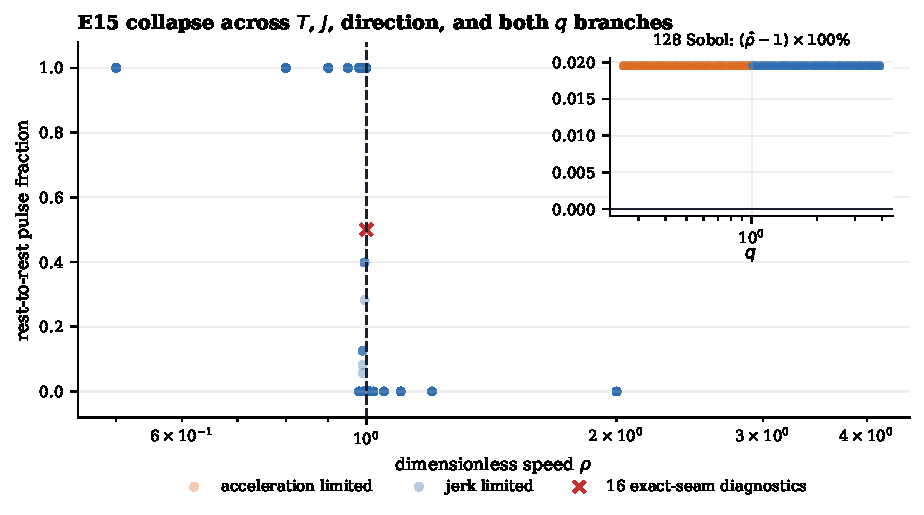
\includegraphics[width=\textwidth]{figures/generated/fig3_e15_collapse.pdf}
 \caption{E15 dimensionless collapse. Required cells from both analytic branches switch across $\rho=1$ after varying period, jerk, and direction. The red marker denotes 16 coincident exact-seam diagnostics, all of which produced native failures in Ruckig~\RuckigVersion. The inset shows the small positive error of all 128 Sobol threshold estimates.}
 \label{fig:e15-collapse}
\end{figure*}

The exact seam must be read differently. All \EFifteenSeamCount{} cells at $q=1,\rho=1$ produced a native solver failure. They are shown in \cref{fig:e15-collapse} rather than dropped. Because the analytic profile topology changes at $q=1$ and one-period feasibility is tight at $\rho=1$, this coordinate combines two boundaries. The experiment does not localize a software defect or prove that a deadband is mathematically necessary there. It establishes a reproducible numerical behavior of version \RuckigVersion{} at an exact seam. The required grid excludes these diagnostics by design, so their failure neither changes the theorem nor gets counted as successful boundary confirmation.

The phase map also clarifies why endpoint RMSE alone would be misleading. Below the boundary, many cells exactly reach the scheduled endpoint and report an exact profile, yet their pulse fraction and endpoint-stop fraction are one. Above the boundary, the one-period rest target is infeasible and the profile cannot complete the same repeated stop. The transition is thus about the reachable terminal state, not loss of position accuracy. This links the theory to the observed mechanism without treating the theorem as a statement about solver policy.\claimtag{C1}

Finally, the cross-limit collapse supports the monotonic implication in \cref{cor:monotonic}. The same physical reference speed can move from $\rho>1$ to $\rho<1$ when $A$, $J$, or $T$ increases. In the tested setting, such a change makes the unintended per-tick rest request reachable. This is why tuning limits can move the symptom while leaving its semantic cause untouched.


\section{Causal Remedy and Ablations}
\label{sec:remedy-results}

\subsection{Velocity coefficient identifies the active cause}

The velocity-scale intervention in \cref{fig:e16-ablation}a produces a structured dose response. At $\lambda=0$, the velocity field carries the same zero terminal velocity as P-only and retains high ripple. Moving $\lambda$ toward one progressively reduces ripple; the matched value $\lambda=1$ reaches zero median ripple. Overshoot at $1.25$ reintroduces variation, while the wrong sign $\lambda=-1$ is substantially worse. This shape is evidence against an explanation based on merely adding another target component. The component must carry the derivative consistent with the intended motion.\claimtag{C3}

\begin{figure*}[t]
 \centering
 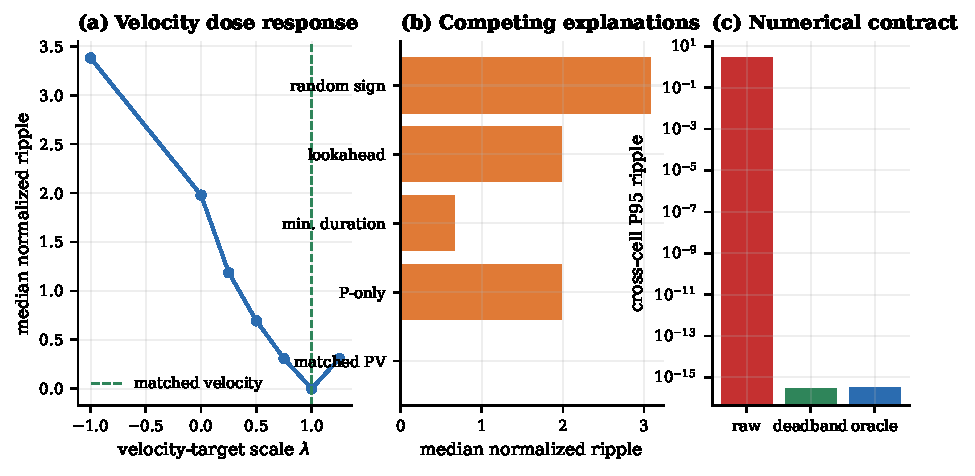
\includegraphics[width=\textwidth]{figures/generated/fig4_e16_ablation.pdf}
 \caption{E16 causal interventions. (a) Velocity-target scale $\lambda$ yields a dose response with an exact minimum at the matched value. (b) Random sign, position lookahead, minimum duration, and P-only retain nonzero median ripple; the bar pools the settings within each tested alternative. (c) Raw \FutureOOne{} leaves a microscopic cross-cell P95 residual, whereas the fixed deadband and oracle PV meet the exact criterion.}
 \label{fig:e16-ablation}
\end{figure*}

Across all \ESixteenArmCount{} arms, matched/oracle PV has median normalized ripple zero and eliminates the rest-to-rest pulse in every tested primary cell. The pooled wrong controls have median ripple \ESixteenWrongRipple. These are exact-profile statements in a single-axis grid; they do not establish that PV is a universal optimum for arbitrary references or objectives. They do establish that matched velocity is the only tested intervention that reproduces the invariant continuation throughout this grid.\claimtag{C3}

\subsection{Lookahead and duration are not exact substitutes}

None of the tested position-lookahead horizons $0,1,2,$ or $5$ reproduces the matched-PV exact profile in every E16 cell. Lookahead changes the requested displacement but leaves the endpoint velocity at zero. It can therefore alter pulse duration or move a configuration across the reachability boundary without repairing the contradiction with constant motion. Likewise, none of the minimum-duration settings off, $T$, $2T$, or $5T$ is an exact equivalent. A duration constraint can delay completion, but it does not require the terminal velocity to equal $\vref$.\claimtag{C4}

These are bounded negative conclusions. A different preview law, a controller that interprets duration differently, or a coupled optimization over several future states could produce another result. E16 shows that the specific tested alternatives do not explain the matched-PV outcome and should not be described as interchangeable repairs. The result is strongest at the level of exact profiles; comparing endpoint positions alone would make several alternatives appear unnecessarily similar.

% Generated; do not edit.
\begin{table*}[t]
\centering
\caption{Causal interpretation of tested target contracts. ``Exact'' refers to the preregistered within-period profile criterion in E16, not only endpoint position.}
\label{tab:causal-ablation}
\small
\begin{tabularx}{\textwidth}{@{}p{0.18\textwidth}p{0.17\textwidth}X X@{}}
\toprule
Intervention & Exact in all tested primary cells? & Observed result & Bounded interpretation \\
\midrule
P-only $(p^\star,0,0)$ & No & repeated rest-to-rest pulses & terminal-state mismatch \\
Matched/oracle PV & Yes & zero median ripple & tested exact remedy \\
Velocity scale $\lambda\ne1$ & No & dose response; wrong sign is worse & derivative value matters \\
Random velocity sign & No & median ripple $3.2007$ & not an extra-DOF effect \\
Position lookahead $0,1,2,5$ & No & no tested horizon reproduces PV & not an exact substitute here \\
Minimum duration off/$1,2,5T$ & No & no tested duration reproduces PV & timing alone is insufficient here \\
Raw Future-O1 & No & microscopic cross-cell residual & implementation-level numerical interaction \\
Future-O1 + $10^{-10}$ deadband & Yes & exact within E16 criterion & tested numerical contract \\
Matched PVA at constant speed & Equivalent to PV & 80 coordinates agree in primary metrics & $a_{\rm ref}=0$ negative control \\
\bottomrule
\end{tabularx}
\end{table*}


\subsection{Causal construction and numerical deadband}

Raw \FutureOOne{} is algebraically exact for the affine schedules in E16, yet floating-point target values create a microscopic residual in some cross-branch cells. The raw method therefore fails the preregistered P95 exactness criterion even though it eliminates macroscopic pulses. Conditioning target velocities within \RecordedDeadband{} of the intended value restores the exact profile in all tested cells. We interpret this as part of the tested numerical contract with Ruckig~\RuckigVersion, not as a universal mathematical requirement for derivative targets.\claimtag{C12}

The recorded fixed-grid targets provide an independent magnitude check on that conditioning scale. Among \RecordedCycleCount{} raw target-velocity entries, exactly \RecordedZeroTargetCount{} are zero, and the smallest nonzero magnitude is \RecordedMinimumNonzeroTarget. It exceeds the E16 deadband by more than an order of magnitude. Applying the same deadband would therefore leave every nonzero recorded target unchanged; no recorded performance gain is being manufactured by truncating small but meaningful velocities. This check establishes target-sequence equivalence, while a later clean replay remains the release-level provenance gate.

\subsection{Matched acceleration as a negative control}

A05 compares matched PV and PVA on constant-speed coordinates. For each finite-difference stencil, the primary stop-and-go metrics agree across \PVAPVEquivalentCoordinateCount{} paired coordinates to the declared tolerance. This is expected from the motion: the matched acceleration is zero, so PVA supplies no additional derivative information. The result is a useful negative control for the mechanism but does not imply that acceleration targets are generally useless. Indeed, nonconstant reference motion and arbitrary target-state OTG are precisely settings in which nonzero target acceleration can matter~\cite{berscheid2021ruckig}.\claimtag{C8}

Together, the interventions support a causal chain: zero terminal velocity produces the pulse when rest-to-rest is reachable; the correct velocity coefficient removes it; wrong values do not; position preview and timing constraints are not exact substitutes in the tested grid; and a history-only construction retains the effect after an implementation-specific numerical conditioning step.

\section{Robustness Within the Tested Envelope}
\label{sec:robustness-results}

\subsection{Frozen condition-wise holdout}

The local-polynomial candidate was selected using development seeds only and then frozen. On the holdout, all \ESeventeenWorkPairCount{} paired cells improve normalized velocity ripple, and all 11 declared conditions pass their condition-wise criteria. The aggregate near-unity reductions under clean, quantized, delayed, dropout, and timestamp-jitter inputs are less informative than the weakest condition. At position noise $0.1$ of a position step, the median reduction is \ESeventeenWeakMedianPercent, the minimum across paired cells is \ESeventeenWeakMinimumPercent, and all \ESeventeenPairPerCondition{} pairs still improve. Reporting this weakest result avoids allowing easy conditions to dominate a pooled median.\claimtag{C6}

\begin{figure*}[t]
 \centering
 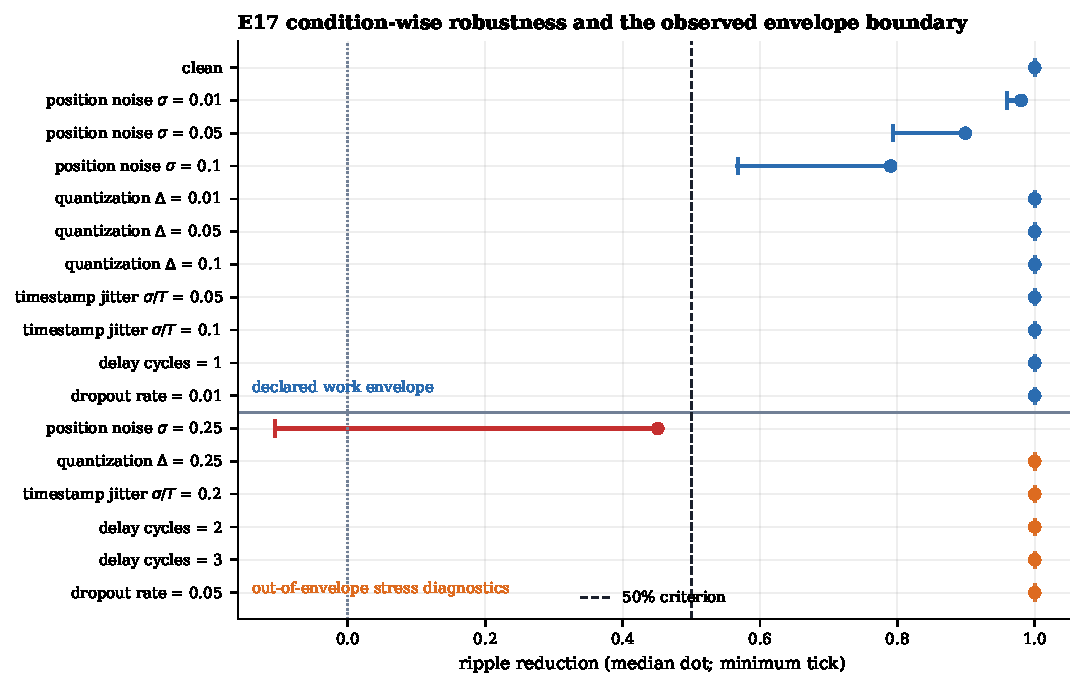
\includegraphics[width=\textwidth]{figures/generated/fig5_e17_robustness.pdf}
 \caption{E17 condition-wise results. Dots show medians and ticks show minima over \ESeventeenPairPerCondition{} paired seed--configuration cells per condition. The first 11 rows form the declared work envelope. The remaining six rows are stronger stress diagnostics. Position noise $0.25$ crosses the 50\% median criterion and contains one cell with negative reduction, exposing an observed boundary rather than supporting extrapolation.}
 \label{fig:e17-robustness}
\end{figure*}

The paired design matters. E17 contains \ESeventeenHoldoutRowCount{} holdout method rows because it evaluates multiple candidate methods and baselines, but those rows are not independent tasks. The confirmatory statement uses matched baseline--candidate pairs indexed by perturbation, $q$, $\rho$, and seed. We report exact condition counts and distributions rather than treating all internal rows as independent samples or highlighting a bootstrap interval across pseudo-replicated solver calls.

\subsection{Stress diagnostics expose the envelope boundary}

The six stronger perturbations were retained precisely to test how the selected observer fails outside the declared envelope. Five remain near complete ripple suppression. Position noise $0.25$, however, has median reduction \ESeventeenStressMedianPercent, below the $50\%$ condition criterion, and a minimum of \ESeventeenStressMinimumPercent. Although \ESeventeenStressImprovedCount{} of \ESeventeenPairPerCondition{} cells still improve, one becomes worse than its P-only baseline. This is not a failed preregistered holdout because the condition was never in the work envelope. It is a useful domain boundary that constrains the claim: the causal PV construction is robust \testedEnvelope, not under arbitrary position noise.\claimtag{C6}

The result also separates the target-state remedy from observer quality. Proposition~\ref{prop:matched-pv} assumes a matched velocity is available. A noisy causal estimator may fail to supply it closely enough. The resulting loss of performance does not reinstate the zero-velocity P-only contract as correct; it shows that derivative estimation and target semantics are two different design problems.

\subsection{Nonconstant synthetic trajectories}

All \ESeventeenSyntheticCount{} held-out synthetic trajectories pass the trajectory-level guardrails. They cover constant, ramp, sine, chirp, and reversal families, and the worst ripple reduction is \ESeventeenSyntheticWorstPercent. This extends the observed mechanism beyond constant schedules in the tested generator: carrying a causal velocity target remains beneficial when the intended derivative varies smoothly and changes sign.\claimtag{C7}

The extension remains synthetic. The trajectories share the single-axis kinematic model and generated disturbance process. They do not contain robot dynamics, contact, coupled joint limits, synchronization, sensor calibration errors, or a task distribution sampled from deployed robots. We therefore avoid terms such as robot generalization. The correct description is a nonconstant synthetic holdout inside a declared experimental design.

\subsection{Irregular timestamps: a visible negative result}

The recorded replay has source intervals from approximately $8.98$ to $11.09$ ms. Fixed-grid \FutureOOne{} rejects this horizon because it supports exactly one nominal step, which is the safe behavior under the information contract. The timestamp-aware local-polynomial method completes, but its RMSE is \RecordedLocalPolyRMSE, worse than the scheduled-P value \RecordedBaselineRMSE. It also leaves the same 20 ms integer observed lag. This replay is not an independent holdout and does not overturn the fixed-grid A04 result; it shows that the current irregular-timestamp observer has not solved the recorded case.\claimtag{C13}

\Cref{tab:robustness} consolidates the work-envelope result, the separately
labeled stress diagnostics, the synthetic trajectories, and this negative
replay without pooling their statistical units.

\section{Recorded-Trajectory Case Study}
\label{sec:recorded-results}

\subsection{Fixed-grid target-contract comparison}

On the one recorded fixed-grid waveform, scheduled P has position RMSE \RecordedBaselineRMSE, integer observed lag 20 ms, and sub-sample lag \RecordedPSubsampleLag. PV \FutureOOne{} at the vendor limits reduces RMSE to \RecordedPVRMSE, a \RecordedPVReductionPercent{} reduction on the same waveform. Its integer lag is \RecordedPVLag{} and its sub-sample lag is \RecordedPVSubsampleLag. The local trace in \cref{fig:recorded-case} shows a region selected by a deterministic rolling error-difference rule: PV follows the changing reference more closely than P without implying that every local interval improves.\claimtag{C9}

\begin{figure*}[t]
 \centering
 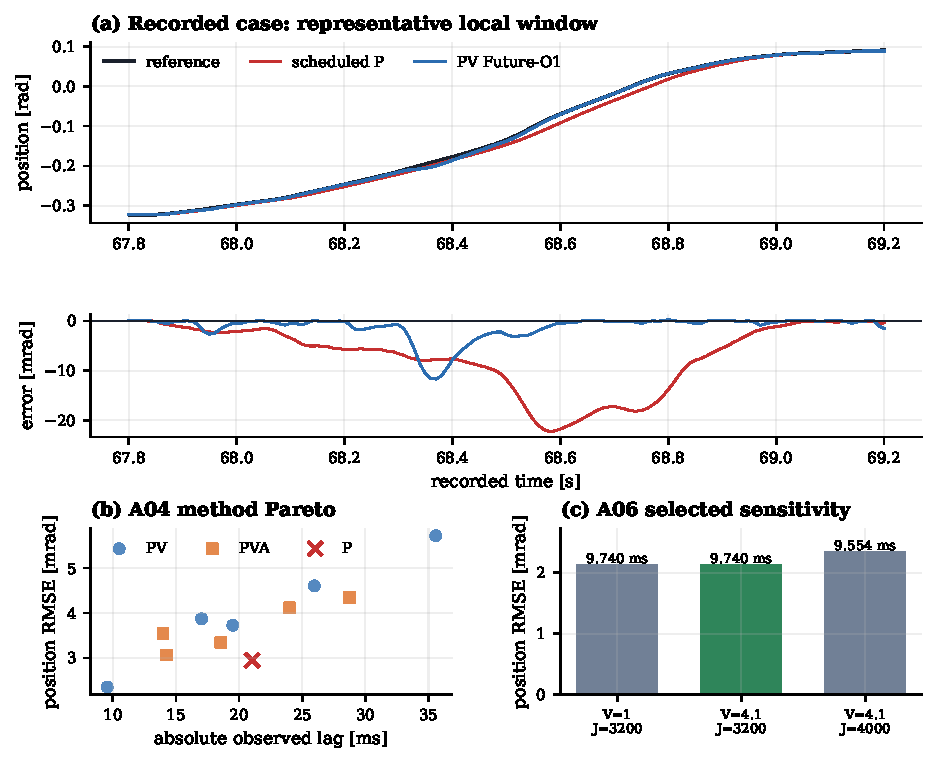
\includegraphics[width=\textwidth]{figures/generated/fig6_recorded_case.pdf}
 \caption{Recorded fixed-grid case study. (a) Reference, scheduled P, and PV \FutureOOne{} with position errors over a representative local window. (b) A04 RMSE--sub-sample-lag comparison for five PV and five PVA stencils, with P shown as a cross. (c) A06 sensitivity for the two performance-equivalent $J=3200$ settings and the $J=4000$ vendor reference. Lags are waveform-alignment diagnostics.}
 \label{fig:recorded-case}
\end{figure*}

PVA \FutureOOne{} does not improve this case. Its RMSE is \RecordedPVALRMSE, approximately \RecordedPVAIncreasePercent{} above scheduled P, while its integer lag is \RecordedPVALag{} and sub-sample lag is \RecordedPVASubsampleLag. This does not conflict with arbitrary-target-state OTG or with the value of acceleration targets in dynamic motion. It says that the particular causal acceleration construction and recorded waveform provide no net benefit under the current limits. Together with the constant-speed equivalence in A05, it prevents the acceleration field from being credited merely because it adds another component.\claimtag{C8}

One offline-host deadline miss occurred in the selected PV run, corresponding to one of \RecordedCycleCount{} evaluated cycles. Core kinematic constraints, solver completion, and target projection guardrails pass. Deadline is not used as the primary scientific gate, and this isolated diagnostic is not evidence of hardware real-time schedulability. A real-time claim would require a specified processor, operating system, scheduling policy, complete controller stack, and worst-case timing protocol.

\subsection{Vmax attribution}

A03 intervenes on the runtime velocity limit, changing it from $4.1$ to $10\ \mathrm{rad\,s^{-1}}$ for the same recorded inputs and PVA methods. For Future-O1, the log-ratio interaction of the PVA/P RMSE relationship is \VmaxInteraction, and acceleration projection counts remain unchanged. Across the tested stencils, relaxing runtime $V_{\max}$ does not remove the PVA deficit. The tested velocity condition becomes nonbinding while acceleration-related projection persists. We therefore reject runtime $V_{\max}$ as the explanation for the observed PVA degradation in this input and limit range. We do not claim that velocity limits are irrelevant in other tasks.\claimtag{C11}

\subsection{Best-tested VAJ setting}

A06 performs the second-stage engineering search after PV \FutureOOne{} has been selected. The deployment recommendation preserves the vendor velocity limit and uses $V/A/J=4.1/8.2/3200$. It achieves RMSE \RecordedBestRMSE, an improvement of \RecordedBestReductionPercent{} over scheduled P, with 10 ms integer lag, \RecordedBestSubsampleLag{} sub-sample lag, and zero target projection. The performance-equivalent $V=1$ setting has six projected targets, which is why it is not the deployment recommendation.\claimtag{C10}

The selected acceleration $A=8.2$ lies on the tested grid boundary, so the result is boundary-censored. It is the \emph{best tested} configuration, not a global optimum. Relative to the $J=4000$ vendor reference, $J=3200$ lowers RMSE by about \RecordedBestVsVendorReductionPercent{} while increasing sub-sample observed lag by approximately \RecordedBestLagTradeoff. The two co-primary metrics therefore retain a small trade-off that an integer-lag-only report would hide.

% Generated; do not edit.
\begin{table*}[t]
\centering
\caption{Recorded fixed-grid case study. Lags are observed waveform lags, not wall-clock latency. The deadline column is an offline-host guardrail.}
\label{tab:recorded}
\small
\begin{tabular}{@{}llllrrrrl@{}}
\toprule
Contract & Observer & $V/A/J$ & Role & RMSE [rad] & lag [ms] & sub-sample [ms] & projection & deadline \\
\midrule
P & none & $4.1/8.2/4000$ & baseline & 0.002951 & 20 & 21.029 & 0 & pass \\
PV & Future-O1 & $4.1/8.2/4000$ & method selection & 0.002352 & 10 & 9.554 & 0 & 1 miss \\
PVA & Future-O1 & $4.1/8.2/4000$ & negative result & 0.003536 & 10 & 13.976 & 0 & pass \\
PV & Future-O1 & $4.1/8.2/3200$ & best tested & 0.002129 & 10 & 9.740 & 0 & diagnostic \\
\bottomrule
\end{tabular}
\end{table*}

% Generated; do not edit.
\begin{table*}[t]
\centering
\caption{Robustness and negative controls. The recorded replay is diagnostic and is not an independent holdout.}
\label{tab:robustness}
\small
\begin{tabularx}{\textwidth}{@{}p{0.16\textwidth}p{0.17\textwidth}p{0.22\textwidth}X X@{}}
\toprule
Evidence & Evaluation unit & Result & Supports & Does not support \\
\midrule
E17 work envelope & 11 conditions, 1,320 pairs & all improve; weakest median 79.03\% & robustness in declared envelope & robot generalization \\
E17 stress diagnostics & 6 conditions, 720 pairs & noise 0.25 median 45.13\%, min. -10.63\% & visible envelope boundary & universal noise robustness \\
Synthetic trajectories & 20 trajectories & 20/20 pass; worst 98.67\% & tested nonconstant references & physical-task coverage \\
Recorded irregular replay & one waveform & local poly 0.003308 vs. P 0.002951 rad & explicit negative result & irregular-sampling remedy \\
\bottomrule
\end{tabularx}
\end{table*}


\Cref{tab:recorded} reports the recorded metrics and guardrails together. The
case study supports the mechanism at deployment-relevant scale without becoming
a generalization experiment. It contains one axis, one waveform, and no physical
plant. The causal comparison is A04's same-waveform target-contract intervention.
The additional A06 gain is an engineering selection layered on top; it must not
be attributed solely to the matched velocity target.

\section{Discussion and Limitations}
\label{sec:discussion}

\subsection{The result is about state semantics}

The central result is not a recommendation to tune Ruckig or to append a velocity field indiscriminately. It is a statement about the semantics of a moving target. A complete OTG target describes how the trajectory should arrive, not only where. Repeatedly pairing a moving position with zero terminal derivatives asks for repeated stops. When the displacement falls inside the one-period rest-to-rest reachable set, an exact solver can satisfy that request and produce a waveform that is undesirable for the application. The endpoint is correct; the continuous-motion contract is not.\claimtag{C1}

This perspective explains why the matched velocity intervention is causal. The zero-jerk continuation in \cref{prop:matched-pv} is feasible because its terminal derivative matches the invariant motion. E16 then shows that the tested solver realizes that continuation, while wrong coefficients, random signs, tested position preview, and tested duration settings do not. The experiment does not prove logical uniqueness among all possible command-shaping schemes. It shows that the derivative value, rather than the mere presence of another input or more time, accounts for the exact profile in the declared grid.

The dimensionless boundary turns a qualitative interface warning into a quantitative diagnostic. For a candidate constant-speed command, an engineer can compute $q$, $\vcrit$, and $\rho$ before running an OTG. If $\rho\le1$, per-tick rest is reachable under the theorem assumptions. This does not guarantee that every solver stops, but it identifies when a zero-velocity terminal contract makes stopping physically feasible. The monotonicity result also prevents a common misdiagnosis: loosening acceleration or jerk limits may enlarge the stop region. A limit change that suppresses the visible artifact at one speed is not evidence that the contract is correct.

A practical audit can therefore proceed in four layers. First, inspect the complete target tuple actually delivered to the generator after defaults, unit conversions, projections, and startup handling; documentation of the desired position alone is insufficient. Second, compare the terminal derivatives with invariants of the intended reference, using $\rho$ as a screening calculation for locally constant motion. Third, sample or integrate the committed within-period profile and test velocity minima, ripple, terminal stops, and constraint activity in addition to endpoint error. Fourth, perturb one semantic component at a time while holding the input waveform and limits fixed. This order helps distinguish a target-state mismatch from an estimator delay, constraint projection, solver failure, or downstream plant response. It also discourages tuning several limits and observers simultaneously and then assigning the combined improvement to a single cause. The present E15--E17 sequence is one concrete implementation of that audit, not a mandated benchmark format.

\subsection{Endpoint metrics can certify the wrong behavior}

The experiments demonstrate a broader evaluation lesson. Sampling a command only at tick boundaries can erase the behavior most relevant to the mechanism. A pulse can start and end at the scheduled positions while reaching zero velocity inside every period. Position RMSE and integer lag remain useful tracking summaries, especially for the recorded case, but they are not mechanism identifiers. Exact-profile velocity ripple, near-zero fraction, pulse fraction, and endpoint stops answer a different question.

This is why the paper does not combine all evidence into one score. E15 and E16 ask whether a precise within-period profile occurs. E17 asks how much ripple reduction survives declared perturbations. A04 and A06 ask about recorded waveform RMSE and observed alignment. The metrics are connected by the target-state hypothesis but retain their own units and statistical interpretation.

\subsection{Numerical seams and deadbands}

Two numerical phenomena deserve separate treatment. First, all 16 E15 cells exactly at $q=1,\rho=1$ fail natively. This coordinate is simultaneously an analytic regime seam and a tight feasibility boundary. We report the failure but do not identify its internal cause or generalize it beyond Ruckig~\RuckigVersion. Second, raw \FutureOOne{} leaves microscopic target differences that prevent exact matching in some E16 cells; a fixed $10^{-10}\ \mathrm{rad\,s^{-1}}$ deadband restores the declared profile. This conditioning is part of the tested implementation contract, not a theorem about all floating-point OTG algorithms.\claimtag{C12}

The recorded target audit reduces one concern about the deadband. The smallest nonzero raw target is \RecordedMinimumNonzeroTarget, so the E16 threshold changes no nonzero target in that sequence. It does not, however, establish an optimal deadband for noisy data. A deployment should derive conditioning from units, estimator error, solver tolerance, and the smallest meaningful velocity, then test it at the relevant version and precision.

\subsection{Observers do not inherit the proposition}

The matched-PV proposition assumes the correct velocity. A causal application must estimate or otherwise obtain that derivative. On a fixed grid, \FutureOOne{} is transparent and affine-exact. Under E17's generated noise and timing model, a development-selected local polynomial is more robust. At stronger position noise, its median reduction drops below the declared criterion and one paired cell degrades. On the irregular recorded timestamps, the same local-polynomial approach is worse than scheduled P. These results are consistent: the target contract may be structurally correct while a particular observer is poorly matched to a data regime.\claimtag{C5}\claimtag{C6}\claimtag{C13}

No universal observer is claimed. Better irregular-grid estimators could use timestamp-aware state-space models, regularized differentiation, task bandwidth priors, or uncertainty-aware target conditioning. Such changes would require new development and a new independent holdout; they cannot be selected retrospectively from the current negative replay.

\subsection{Recorded and deployment limits}

The recorded study is deliberately called a case study. It contains one axis and one waveform, so the reductions of \RecordedPVReductionPercent{} for method selection and \RecordedBestReductionPercent{} after VAJ selection are descriptive for that case. The A06 acceleration coordinate is boundary-censored, and its $4.1/8.2/3200$ recommendation is best tested rather than globally optimal. The PVA result is similarly local: it does not justify the statement that PVA is generally harmful or useless.\claimtag{C8}\claimtag{C10}

Observed waveform lag is not latency. Cross-correlation describes the relative alignment of generated and reference sequences. It contains effects of target age, filtering, prediction, and trajectory dynamics, but it is not the elapsed time of the software pipeline. The one offline-host deadline miss is reported as a guardrail and prevents a real-time claim. Hardware schedulability requires a separate measurement campaign. Likewise, A03 rejects $V_{\max}$ attribution only for the tested waveform, stencils, and limits.\claimtag{C11}

\subsection{Missing physical and multi-axis validation}

The software model omits actuator dynamics, feedback, friction, quantized encoders, communication, and structural vibration. A physical plant can attenuate or amplify the exact OTG profile. The theorem is single-axis and does not address synchronization across degrees of freedom, Cartesian path error, coupled torque limits, or interactions between independently estimated derivatives. Existing OTG and safe-reaction literature demonstrates why these issues matter in robotic systems~\cite{berscheid2021ruckig,haddadin2008collision,lange2016path}.

A future multi-axis hardware module should preserve C1--C13 and test rather than rewrite them. At minimum it should compare same-waveform P and matched-PV contracts on several axes and speeds spanning $\rho<1$ and $\rho>1$, record commanded and measured states at the servo rate, report synchronization and Cartesian errors, and measure worst-case execution time on the target controller. Until then, the defensible arXiv claim is theory plus single-axis software confirmation plus one recorded case study.

\section{Conclusion}
\label{sec:conclusion}

A moving position stream paired with zero terminal derivatives can turn jerk-limited online trajectory generation into repeated rest-to-rest motion. We derived the maximum one-period rest-to-rest displacement and expressed its reachability boundary as $\rho=1$ with an acceleration-limited and a jerk-limited branch. The theorem predicts feasibility; E15 separately confirms the observed transition for Ruckig~\RuckigVersion{} away from a fully reported numerical seam.

A matched velocity target removes the structural contradiction by admitting an invariant zero-jerk continuation. Causal interventions identify the velocity value, rather than generic preview or extra duration, as the active tested remedy. Frozen holdout experiments support robustness \testedEnvelope{} and expose a stronger-noise boundary. One recorded fixed-grid case improves both RMSE and observed waveform lag, while an irregular-timestamp replay remains a visible negative result.

The engineering lesson is to treat derivative targets as part of the command's meaning. Endpoint position accuracy cannot certify continuous-motion quality. Applications should specify a target state consistent with intended motion, state the causal information contract used to construct it, and validate within-period profiles as well as sampled tracking metrics. These conclusions remain single-axis and software-based pending multi-axis physical validation.



\appendix
\section{Complete Rest-to-Rest Boundary Proof}
\label{app:proofs}

This appendix supplies the optimality step compressed in \cref{thm:rest-boundary}. Let $\mathcal U$ be the set of measurable jerks satisfying $\abs j\le J$ whose integrated acceleration satisfies $\abs a\le A$ and whose terminal velocity and acceleration are zero. This set is convex. For fixed $T$, $p(T)$ is linear in $j$, so a maximum occurs at an extreme feasible control. Pontryagin's maximum principle gives a switching function that is quadratic between acceleration-boundary arcs. Consequently, an extremal jerk saturates at $\pm J$ off those arcs and is zero only while $a=\pm A$. This is the familiar bang--boundary--bang structure; the argument is used here only for the scalar fixed-time linear system, not asserted for the full OTG implementation.

Because $v(T)=v(0)=0$, $\int_0^T a(t)\,dt=0$, and
\begin{equation}
 d=p(T)-p(0)=-\int_0^T t\,a(t)\,dt.
 \label{eq:proof-displacement}
\end{equation}
If $a(t)$ is feasible, then $-a(T-t)$ is feasible and has the same displacement. Convex averaging therefore yields an optimal representative satisfying $a(t)=-a(T-t)$. Its first half is nonnegative for positive optimal displacement, and the second half is the sign-reversed time reflection. Any negative segment in the first half can be removed and reallocated to an earlier positive saturated segment without violating the endpoint integral, increasing \cref{eq:proof-displacement}. Thus the first half is the largest nonnegative acceleration pulse that starts and ends at zero under $A$ and $J$.

Write $H=T/2$. If $A\ge JH/2=JT/4$, the acceleration bound is inactive. The maximum pulse ramps with $+J$ for $H/2$ and with $-J$ for $H/2$:
\begin{equation}
 a(t)=
 \begin{cases}
 Jt,&0\le t\le T/4,\\
 J(T/2-t),&T/4<t\le T/2.
 \end{cases}
 \label{eq:triangular-acceleration}
\end{equation}
The midpoint velocity is the triangle area,
\begin{equation}
 v(T/2)=\frac{1}{2}\frac{T}{2}\frac{JT}{4}=\frac{JT^2}{16}.
\end{equation}
The first-half acceleration is symmetric about $T/4$, so $v(t)+v(T/2-t)=v(T/2)$. Integrating the two halves of the full symmetric velocity profile gives
\begin{equation}
 d_{\max}=\frac{T}{2}v(T/2)=\frac{JT^3}{32}.
\end{equation}

If $A<JT/4$, set $h=A/J<T/4$. The maximal first-half pulse is
\begin{equation}
 a(t)=
 \begin{cases}
 Jt,&0\le t<h,\\
 A,&h\le t\le T/2-h,\\
 J(T/2-t),&T/2-h<t\le T/2.
 \end{cases}
 \label{eq:trapezoidal-acceleration}
\end{equation}
Its area is
\begin{equation}
 v(T/2)=Ah+A(T/2-2h)=\frac{AT}{2}-\frac{A^2}{J}.
\end{equation}
The same symmetry yields
\begin{equation}
 d_{\max}=\frac{T}{2}v(T/2)=\frac{AT^2}{4}-\frac{A^2T}{2J}.
\end{equation}
Dividing by $T$ gives \cref{eq:vcrit}. The maximum velocity of either profile is its midpoint value $2\vcrit$; hence $V\ge2\vcrit$ makes the velocity constraint inactive.

For completeness, inserting a zero-acceleration cruise by shortening each acceleration pulse cannot increase displacement. In the jerk-limited case, a pulse with ramp duration $h\le T/4$ yields $d(h)=Jh^2(T-2h)$, whose derivative $2Jh(T-3h)$ is positive throughout $0<h\le T/4$. In the acceleration-limited case, a positive pulse of duration $L\le T/2$ with fixed ramps $h=A/J$ yields $d(L)=A(L-h)(T-L)$, whose derivative $A(T-2L+h)$ is positive on the feasible interval. Thus both optima use the full half-period pulse described above.

Finally, multiplying the complete signed trajectory by $\alpha=\abs d/d_{\max}\in[0,1]$ preserves the endpoint conditions and weakens every bound. A sign flip reaches negative $d$. This proves reachability for the full interval $[-\dcrit,\dcrit]$ and completes \cref{thm:rest-boundary}.


\section{Metrics and Causal Algorithms}
\label{app:metrics}

For cycle $k$, let $v_k(\tau)$ be the exact solver profile on $\tau\in[0,T]$. A rest-to-rest pulse indicator requires both endpoint velocities to be below the declared numerical tolerance, nontrivial within-period motion, and exact profile availability. Pulse fraction is the mean indicator over valid cycles; event rate divides the number of pulse onsets by evaluated duration. Endpoint-stop fraction tests $\abs{v_k(T)}$, while near-zero cycle fraction tests whether the exact profile approaches zero inside the committed interval.

Normalized velocity ripple is
\begin{equation}
 r_k=\frac{\max_{\tau\in[0,T]}v_k(\tau)-\min_{\tau\in[0,T]}v_k(\tau)}{\abs{\vref}},
\end{equation}
with sign-consistent handling for negative reference motion. E17 ripple reduction for paired baseline $b$ and candidate $c$ is $(r_b-r_c)/r_b$. The condition summary reports the median, minimum, and positive-improvement fraction across the \ESeventeenPairPerCondition{} paired $q$--$\rho$--seed cells. A pair is the unit; individual solver rows are not treated as independent samples.

Recorded position RMSE over the evaluation index set $\mathcal K$ is
\begin{equation}
 \operatorname{RMSE}=\sqrt{\frac{1}{\abs{\mathcal K}}\sum_{k\in\mathcal K}(p_k-P[k])^2}.
\end{equation}
Integer observed lag maximizes discrete cross-correlation over the declared lag window. Sub-sample lag fits a quadratic through the maximizing correlation sample and its two neighbors. Neither metric reads per-cycle software timestamps, so neither is labeled latency.

\FutureOOne{} is evaluated only when the target horizon equals one nominal fixed-grid period. At startup, insufficient history invokes the declared startup behavior. The E16 conditioned version replaces target velocities whose numerical residual from the intended affine value is no larger than $10^{-10}\ \mathrm{rad\,s^{-1}}$. The threshold is held fixed across E16 cells. The E11 audit in \cref{sec:remedy-results} confirms that it would alter no nonzero recorded Future-O1 target.

\section{Full Matrix and Negative-Result Accounting}
\label{app:matrices}

E15 uses $T\in\{2,5,10,20\}$ ms, $J\in\{1000,4000\}$, both directions, nine $q$ levels from $0.25$ to $4$, and fifteen $\rho$ levels from $0.5$ to $2$. The 16 exact $q=1,\rho=1$ seam cells are diagnostic. E16 uses $T\in\{5,10,20\}$ ms, $q\in\{0.5,0.95,1.05,2\}$, and $\rho\in\{0.5,0.9,0.99,1.01,1.1\}$ with the intervention families listed in \cref{sec:protocol}. The generated artifact manifest retains the full CSVs rather than only the plotted aggregates.

E17 has \ESeventeenDevelopmentRowCount{} development rows and \ESeventeenHoldoutRowCount{} holdout method rows. The confirmatory work-envelope summary contains 11 conditions and \ESeventeenWorkPairCount{} paired cells. Six stronger conditions contribute \ESeventeenStressPairCount{} diagnostic pairs. Position noise $0.25$ is the only stress condition whose median falls below the predeclared 50\% threshold; its minimum is negative. The synthetic trajectory set contains four instances from each of five families. The irregular-timestamp replay shares the recorded waveform and is explicitly not counted as an independent holdout.

The negative-result ledger is therefore: 16/16 E15 exact-seam native failures; raw Future-O1 failure of the E16 cross-cell P95 exact criterion; no exact equivalence for tested lookahead or minimum-duration settings; one E17 stress condition below criterion; PVA Future-O1 worse than scheduled P in the recorded case; the A06 acceleration coordinate on the grid boundary; no support for Vmax attribution in A03; and no improvement from the current irregular-timestamp recorded replay. These entries are required evidence, not optional diagnostics.

\section{Reproducibility and Provisional Provenance}
\label{app:reproducibility}

This PDF uses the \texttt{\EvidenceProfile} evidence profile. The machine-readable declaration is \texttt{evidence/provisional.yaml}; every source path, run ID, specification hash, git commit, dirty flag, and source-file SHA256 is recorded there. The freezing script validates those fields and copies only the artifacts required for C1--C13 into \texttt{evidence/frozen/provisional}. Figure, table, and numeric generation reads only that frozen directory. The generated summary and \texttt{numbers.tex} are not independent sources of truth.

The current experiment and analysis manifests report dirty worktrees. This is why the draft carries a first-page notice and why the release validator refuses to create an arXiv package. The present profile is suitable for manuscript review and for detecting narrative, figure, and build defects. It is not release-level experimental provenance.

The reproducible draft sequence is:
\begin{enumerate}[leftmargin=*,itemsep=1pt]
 \item validate and freeze the provisional evidence profile;
 \item generate all figures, tables, number macros, and the artifact summary;
 \item run the evidence and authoring checks;
 \item compile with TeX Live/pdfLaTeX and BibTeX;
 \item compile independently with Tectonic using the generated bibliography;
 \item render the PDF and inspect every page, embedded font, reference, and figure.
\end{enumerate}

For release, E11--E17 and A03--A06 must be refreshed from one clean commit. A release profile with the same schema must reproduce discrete classifications exactly and compare scientific floating-point metrics at relative tolerance $10^{-9}$ and absolute tolerance $10^{-12}$, excluding host-timing fields. Real author metadata, a permanent repository URL, release tag, and user-selected code/data licenses are also required. Only then can the draft marker be disabled and the arXiv whitelist package be generated.



\bibliographystyle{unsrtnat}
\bibliography{references}
\end{document}
